\documentclass[10pt,twocolumn]{article}

% use the oxycomps style file
\usepackage{oxycomps}

% usage: \fixme[comments describing issue]{text to be fixed}
\newcommand{\fixme}[2][]{#2}

% read references.bib for the bibtex data
\bibliography{references}

% suppress colored hyperlinks for uniform appearance
\hypersetup{hidelinks}

% include metadata in the generated pdf file
\pdfinfo{
    /Title (Beyond Keyword Search: Hybrid Retrieval and Domain-Aware Filtering for Federal Procurement on SAM.gov)
    /Author (Aaron Good)
}

% set the title and author information
\title{Beyond Keyword Search: Hybrid Retrieval and Domain-Aware Filtering for Federal Procurement on SAM.gov}
\author{Aaron Good}
\affiliation{Occidental College}
\email{agood@oxy.edu}

\begin{document}

\maketitle

\begin{abstract}
Government procurement totals over \$750 billion annually in the United States, yet discovery remains fragmented across dozens of portals with limited search capabilities. We present a hybrid retrieval system for federal procurement opportunity discovery that fuses TF-IDF lexical matching with transformer-based semantic embeddings, combined with domain-specific filtering by NAICS industry classification, state, and small business set-aside eligibility. Using a corpus of 500 opportunity notices from SAM.gov, we evaluate retrieval quality with standard information retrieval metrics---Precision@10, Recall@10, Mean Average Precision (MAP), and Normalized Discounted Cumulative Gain (NDCG@10)---computed against human relevance judgments across 20 test queries. We compare keyword-only, semantic-only, and hybrid configurations at multiple fusion weights. Hybrid search at equal weighting ($\alpha = 0.5$) achieved the highest NDCG@10 and Recall@10, but the optimal approach varied by query type: conceptual queries favored semantic-heavy weighting, technical queries favored lexical matching, and synonym queries performed best under semantic search alone. SAM.gov already offers keyword search with metadata filtering; what it lacks is semantic retrieval. The hybrid approach addresses this gap, and the per-category results show precisely where and why it matters.
\end{abstract}

\section{Introduction}

Public procurement involves enormous volumes of information driving immense economic value: the U.S. federal government alone awarded over \$750 billion in contracts annually \cite{HigherGov2022}, and procurement contracts account for over 10\% of the U.S. budget \cite{Omari2025}. Each procurement opportunity begins as a notice---a structured listing on a portal like SAM.gov containing a title, agency, industry classification codes, and a description of the work sought. These notices are the discovery layer of federal contracting: a contractor scanning for work reads notices first and requests the full solicitation documents only after finding a relevant listing.

Yet the discovery layer has a specific gap. SAM.gov provides keyword search with boolean operators, wildcard matching, and faceted filtering by North American Industry Classification System (NAICS) code, Product Service Code (PSC), set-aside designation, location, and agency---capabilities that address the structural dimension of procurement search. But the underlying text retrieval is purely lexical, and keyword search consistently fails to match relevant opportunities when different terminology is used. A query about ``automated vehicle guidance'' will miss opportunities described as ``driverless car navigation.'' This vocabulary mismatch is well-documented in information retrieval research, but it is especially acute in procurement, where the same service may be described in bureaucratic, technical, or colloquial terms depending on the issuing agency.

Procurement data carries structural dimensions that compound the text retrieval problem. Each notice has NAICS codes that classify the work by industry, set-aside designations that restrict eligibility by business size, and response deadlines that determine urgency. SAM.gov provides faceted filtering on these fields, but users widely report that the platform's search produces either thousands of irrelevant results or zero results, with rigid literal matching that fails to connect contractor needs to relevant opportunities. A small environmental consulting firm does not merely search for ``environmental remediation''---it searches for opportunities under NAICS 541620 with a small business set-aside, using terminology that may not match the issuing agency's description. The Small Business Administration (SBA) defines size standards for every NAICS code \cite{SBA2024}, tying industry classification directly to contractor eligibility. Addressing procurement discovery requires solving both problems: the vocabulary mismatch in text retrieval and the structural matching of contractor profile to opportunity metadata.

This paper presents a hybrid retrieval system for federal procurement opportunity discovery that addresses both dimensions. The system combines TF-IDF lexical matching with Sentence-BERT semantic embeddings to address vocabulary mismatch, and implements domain-specific filtering---by NAICS code, set-aside status, state, and response deadline---that reflects the regulatory structure of federal contracting. We evaluate the system on a corpus of 500 SAM.gov notices using standard IR metrics computed against human relevance judgments. The contribution is not a novel retrieval algorithm but a domain-specific implementation that unifies semantic text retrieval with procurement-aware filtering, and an empirical investigation of where and why each retrieval component contributes across different query types.

\section{Technical Background}

The retrieval problem in procurement discovery involves matching short, often jargon-laden queries against a heterogeneous corpus of structured metadata and occasional narrative text. No single retrieval paradigm handles all query types: keyword searches miss synonyms, semantic models miss domain codes, and neither incorporates the regulatory metadata that determines whether an opportunity is actually relevant to a given contractor. This section introduces the three retrieval components our system combines and the fusion strategy that unites them.

\subsection{Lexical Retrieval}

Classical information retrieval treats documents as bags of words. Term Frequency--Inverse Document Frequency (TF-IDF) assigns each term $t$ in document $d$ a score proportional to its \textit{term frequency} $tf(t,d)$ and inversely proportional to how often it appears across the corpus:

\begin{equation}
tfidf(t,d) = tf(t,d) \times \log\frac{N}{df(t)},
\end{equation}

where $N$ is the total number of documents and $df(t)$ is the number of documents containing $t$ \cite{Manning2008}. Terms that are frequent in one document but rare overall receive high scores. TF-IDF and its variants underlie most modern search engines \cite{Manning2008}.

Okapi BM25 is a modern scoring function that extends TF-IDF with probabilistic reasoning and document-length normalization \cite{Robertson2009}. In BM25, the score of document $D$ for query terms $q_1, \ldots, q_n$ is:

\begin{equation}
\scalebox{0.9}{$
\text{score}(D,Q) = \sum_{i=1}^{n} IDF(q_i) \cdot \frac{f(q_i, D) \cdot (k_1 + 1)}{f(q_i, D) + k_1 \cdot (1 - b + b \cdot \frac{|D|}{avgdl})}
$}
\end{equation}

where $f(q_i, D)$ is the term frequency of $q_i$ in $D$, $|D|$ is the document length (in words), and $k_1, b$ are tunable parameters \cite{Robertson2009}. The inverse document frequency $IDF(q_i)$ further downweights common terms \cite{Robertson2009}. By default, Elasticsearch (a partially open-sourced search engine with semantic capabilities) and similar search engines use BM25 as a ``Practical Scoring Function,'' combining TF-IDF and normalization for document length \cite{ElasticScoring}.

We use TF-IDF for the lexical retrieval component. While BM25 offers improved handling of document length variation, TF-IDF is sufficient for demonstrating hybrid retrieval, and the semantic component compensates for lexical limitations. TF-IDF ensures domain-specific terms (e.g., regulatory codes, NAICS classifications) are matched precisely if needed.

\subsection{Semantic Search with Embeddings}

Semantic search represents text as continuous vector embeddings. Documents are embedded into a high-dimensional space; queries are embedded into the same space; retrieval is nearest-neighbor lookup \cite{SBERTSemantic}. Documents with similar meaning have nearby embeddings, even if they share no vocabulary. A query for ``renewable energy project'' retrieves an opportunity labeled ``solar and wind power plant'' because the embeddings are close, not because the words match.

Each document is encoded into a fixed-length vector by a \textit{sentence embedding} model. At query time, the query is encoded and the nearest document vectors are returned \cite{SBERTSemantic}.

Large transformer models like BERT produce contextual embeddings but require pairwise processing of query and document, which is impractical at scale. The Sentence-BERT (SBERT) approach \cite{Reimers2019} uses a siamese architecture to compute fixed-size sentence embeddings. Reimers and Gurevych (2019) showed that SBERT makes semantic search practical: ``Finding the most similar pair in a collection of 10,000 sentences requires about 50 million inference computations ($\sim$65 hours) with BERT; our Sentence-BERT reduces this to about 5 seconds while maintaining accuracy from BERT'' \cite{Reimers2019}. We use all-MiniLM-L6-v2 from the Sentence-Transformers library \cite{SBERTHome} because it is small enough to load at startup without a GPU, and 384 dimensions is sufficient for a corpus of this size. Each notice's title, organization, description, and NAICS codes are encoded into a single embedding vector.

Semantic embeddings also support asymmetric tasks, where a short keyword query is matched against longer document embeddings. In this project, we compute document vectors once (offline) and at query time encode the user's query. Retrieval then finds nearest neighbors by cosine similarity in the vector index \cite{SBERTSemantic,ElasticHybrid}. The dense-vector search can capture broad topical matches beyond exact keywords.

\subsection{Comparison and Combination of Lexical and Semantic Search}

TF-IDF and semantic search fail in opposite ways. TF-IDF excels when the query uses the same terms as the document but retrieves nothing when wording differs \cite{Rayo2025}. Semantic search finds paraphrases and near-synonyms but may miss domain-specific terms that matter. A notice requiring ``mil-spec 810G certification'' (for military contracting) scores highly on TF-IDF if the query mentions ``mil-spec''; a semantic model might overlook it. Combining both methods lets lexical search anchor on critical terms while embeddings catch what keywords miss.

Given ranked results from both retrieval methods, hybrid systems must combine scores into a unified ranking. Common approaches include Reciprocal Rank Fusion (RRF), which sums inverse ranks, and convex combination, which computes a weighted sum of normalized scores:
\begin{equation}
\text{score} = \alpha \cdot s_{\text{tfidf}} + (1 - \alpha) \cdot s_{\text{semantic}}.
\end{equation}
We adopt convex combination, evaluating multiple weights ($\alpha = 0.3, 0.5, 0.7$) to determine the optimal balance. Scores are min-max normalized before combination to ensure equal contribution from each component.

\section{Related Work}

\subsection{Government Procurement Data and Opportunity Access}

The World Bank's Global Public Procurement Database aggregates procurement indicators across countries to promote transparency \cite{WorldBank2023}. The U.S. maintains the Federal Procurement Data System and SAM.gov; SAM.gov provides comprehensive faceted filtering by NAICS code, set-aside designation, location, and agency, but the underlying text retrieval remains keyword-based \cite{Omari2025}. Omari et al. compiled 45 years of U.S. federal contract data and noted that users ``primarily access this data through keyword searches'' \cite{Omari2025}. In Europe, the Tenders Electronic Daily portal catalogs EU public contracts and similarly relies on keyword text search. A substantial share of contracting activity occurs through channels not indexed on SAM.gov \cite{HigherGov2022}, and small businesses routinely report difficulty discovering opportunities. Our system adds semantic retrieval to address the vocabulary mismatch that keyword search cannot resolve.

Academic work on procurement analysis tends to focus on policy and economics (e.g., how open data affects competition \cite{Rauter2020,Omari2025}), but technical studies on procurement opportunity search are scarce. One recent project (Rayo et al., 2025) developed a hybrid IR system for regulatory texts, combining BM25 with a fine-tuned Sentence Transformer \cite{Rayo2025}. They reported that the hybrid approach significantly outperformed standalone lexical or semantic methods (e.g., higher Recall@10 and MAP@10) \cite{Rayo2025}, validating the value of a combined strategy. Our work applies the same approach to procurement data.

\subsection{Hybrid Information Retrieval Systems}

Hybrid IR---fusing lexical and semantic signals---is now standard practice in production search systems. Elastic's technical documentation notes that merging keyword and vector results yields ``far better results than either lexical or semantic search would do on their own'' \cite{ElasticHybrid}. Typical hybrid methods combine a keyword query (scored by BM25/TF-IDF) with a semantic (vector) query, then fuse results via techniques like Convex Combination (CC) or Reciprocal Rank Fusion (RRF) \cite{ElasticHybrid}. In CC, normalized scores from each branch are weighted and summed; in RRF, documents are scored by summing $1/(k + \text{rank})$ over ranks from each list \cite{ElasticHybrid}. Elastic's engineers note that RRF has the advantage of not requiring precise weight tuning \cite{ElasticHybrid}. These ideas inform our scoring design; we implement Convex Combination and evaluate multiple weights to determine the optimal balance for procurement data.

Production systems like Elasticsearch now support hybrid search natively, combining BM25 with dense vector queries and offering RRF fusion. We opted for a custom implementation to maintain flexibility over embedding model selection and fusion parameters, and to avoid enterprise licensing requirements.

\section{System Design and Implementation}

\subsection{Architecture Overview}

The search engine comprises four modules: Data Ingestion, Index Construction, Search, and Web Interface. The system ingests notice data from SAM.gov's Opportunities API, storing results in a flat CSV file. At startup, the application builds two parallel in-memory indexes: a TF-IDF sparse matrix for lexical matching and a dense embedding matrix for semantic similarity. User queries are processed through both indexes, and results are fused using convex combination before being presented through a web interface \cite{ElasticHybrid}.

\subsection{Data Ingestion}

The ingestion module fetches solicitation notices from the SAM.gov Opportunities API v2. For each notice, we extract: solicitation title, issuing organization and parent agency hierarchy, NAICS and PSC classification codes, set-aside designation, response deadline and place of performance, and links to full solicitation documents.

SAM.gov publishes several notice types, each with different data characteristics. Solicitations, Presolicitations, and Sources Sought notices are the primary targets for contractor discovery. Combined Synopsis/Solicitation notices from agencies like the Defense Logistics Agency often contain only part numbers and no narrative text. Award Notices describe completed procurements and are irrelevant to opportunity discovery. The ingestion module filters by notice type to ensure corpus quality, defaulting to types that contain text worth searching.

The API returns structured JSON, but full solicitation text---the narrative scope of work and requirements---requires a secondary fetch from a rate-limited endpoint. To manage SAM.gov's daily API quota, ingestion is split into two passes: a metadata pass that retrieves notice listings at one API call per 100 records, and a solicitation text pass that fetches narrative content from linked URLs at one call per notice. Without the split, text fetches consume the quota needed for listing retrieval. Requests use exponential backoff on rate-limit (429) and server error (5xx) responses, with a maximum of three retries per page. If all retries fail, the script saves whatever rows have been collected rather than discarding them. Results are deduplicated by notice ID and stored in a flat CSV file. While a production system might use a relational database, the flat-file approach simplifies deployment and debugging for this prototype.

Corpus construction required deliberate filtering. Of the notice types available through the API, only Solicitations, Presolicitations, and Sources Sought consistently contained the structured metadata needed for meaningful retrieval. The evaluation corpus comprises 500 notices spanning 181 unique NAICS codes, over 60 agencies, and 24 states. The complete solicitation text---available only through SAM.gov's rate-limited description endpoint---was retrieved for 3\% of notices; the remainder are indexed on the structured metadata fields---title, organization, NAICS, PSC, and set-aside---which are populated for 95--100\% of records.

\subsection{Index Construction}

At startup of the application, the system builds two parallel indexes from the CSV data:

\textit{TF-IDF Index:} We use scikit-learn's TF-IDF vectorizer configured with English stopword removal, a maximum vocabulary of 50,000 terms, and unigram/bigram features (n-gram range 1--2). For each document, we concatenate the title, organization name, parent agency path, NAICS codes, PSC codes, and description into a single text field. This combined text is transformed into a sparse TF-IDF vector. Query-time scoring uses cosine similarity.

\textit{Semantic Index:} We encode each document's combined text using the all-MiniLM-L6-v2 model. This produces a dense numpy matrix of 384-dimensional embeddings, normalized to unit length. Because embeddings are pre-normalized, cosine similarity reduces to a simple dot product, enabling efficient computation via matrix multiplication.

Both indexes are held entirely in memory, enabling sub-second query response times. For a corpus of several hundred notices, index construction completes in several seconds on a local machine.

\subsection{Search and Scoring}

When a user submits a query, the system can operate in three modes: keyword-only (TF-IDF), semantic-only, or hybrid.

\textit{Keyword Search:} The query is transformed using the same TF-IDF vectorizer, and cosine similarity is computed against all document vectors. Documents with zero similarity (no term overlap) are excluded.


\textit{Semantic Search:} The query is encoded using the same embedding model. Cosine similarity is computed via dot product against all document embeddings. Documents below a cosine similarity threshold of 0.25 are excluded from results. Without the cutoff, in a corpus where most documents share generic vocabulary (e.g., ``Department of Defense,'' ``contract''), the least-bad match appears artificially strong after normalization.

\textit{Hybrid Search:} Both similarity computations execute over the full corpus. Raw scores from each method are min-max normalized across all documents---not within a pre-selected subset---to ensure each component's scale reflects its actual confidence distribution. The final score uses convex combination:
\begin{equation}
\scalebox{0.88}{$
\text{HybridScore}(D) = \alpha \cdot \text{TF-IDF}_{\text{n}}(D) + (1 - \alpha) \cdot \text{Sem}_{\text{n}}(D)
$}
\end{equation}
where $\text{TF-IDF}_{\text{n}}$ and $\text{Sem}_{\text{n}}$ denote min-max normalized scores for each method.

We evaluate three fusion weights ($\alpha = 0.3$, $0.5$, $0.7$) to determine which balance of lexical and semantic signals produces the best retrieval quality on our test queries. In a corpus where most documents lack full descriptions and are indexed primarily on title and metadata, lexical matching on structured fields (NAICS codes, agency names) carries more discriminative signal than semantic embeddings on short text---and the evaluation bears this out: on technical queries, $\alpha = 0.7$ produced the best results. Documents appearing in only one method's results receive a score of zero for the missing component, naturally penalizing documents that lack cross-method agreement.

\subsection{User Interface}

The web interface uses FastAPI and Jinja2 templates---the simplest way to serve a Python search application without adding framework overhead. Key features include: search mode toggle allowing users to select Hybrid (default), Semantic, or Keyword mode; domain-specific filters including NAICS code (with prefix matching, so ``5416'' returns both 541611 and 541620), set-aside designation (including small business, SBA 8(a) business development, Historically Underutilized Business Zone, Women-Owned Small Business, and Service-Disabled Veteran-Owned Small Business categories), state, and response deadline range; score transparency displaying both component scores (TF-IDF and semantic) alongside the combined score in hybrid mode; and pagination with 10 items per page.

The NAICS filter merits particular attention. Each NAICS code carries an SBA size standard---a revenue or employee threshold that determines whether a firm qualifies as ``small'' for that industry. By filtering on NAICS code, a contractor implicitly filters by size eligibility. The interface presents the twenty most frequent NAICS codes in the corpus as a dropdown with human-readable labels (e.g., ``541620 --- Environmental Consulting''), alongside a text input for arbitrary codes. This is how contractors actually search: not by keyword alone, but by the intersection of what they do and what they are eligible to bid on.

The interface uses a dark theme designed for extended use, with clear visual hierarchy distinguishing metadata (agency, deadline, state, NAICS, set-aside) from description snippets. Figure~\ref{fig:ui} shows the search interface in active use.

\begin{figure}[h]
    \centering
    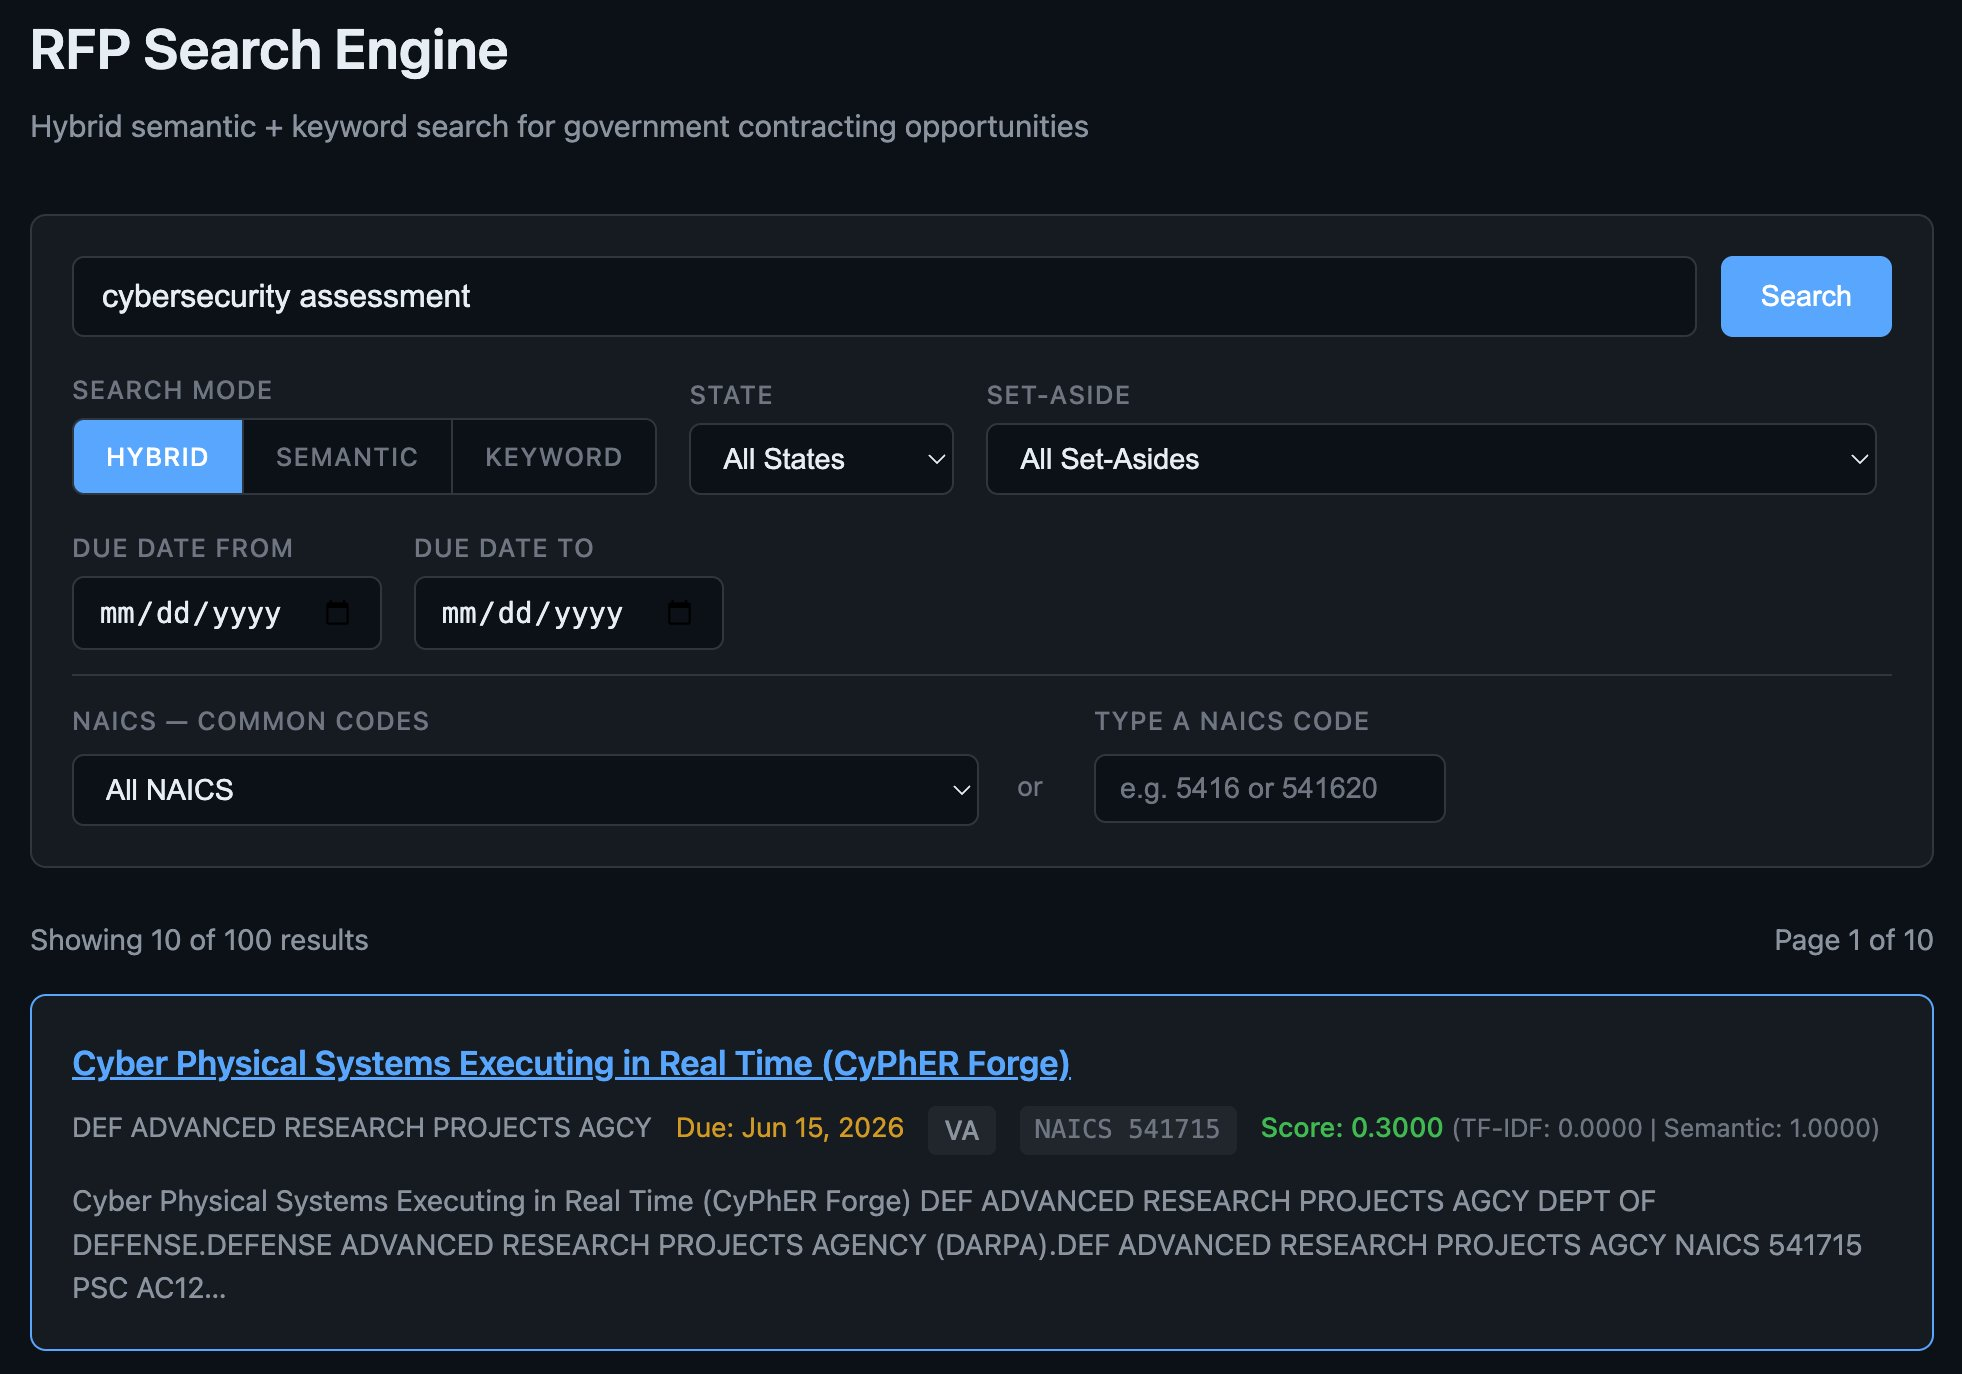
\includegraphics[width=\columnwidth]{ui_screenshot.png}
    \caption{Search interface showing hybrid mode with score transparency and domain-specific filters. Result metadata includes NAICS classification and set-aside designation alongside agency and deadline information.}
    \label{fig:ui}
\end{figure}

\subsection{Design Decisions and Trade-offs}

\textit{TF-IDF vs. BM25:} We use TF-IDF rather than BM25 for the lexical component. While BM25 offers improved handling of document length variation, TF-IDF integrates directly with scikit-learn's vectorization pipeline and is sufficient for demonstrating hybrid retrieval. The semantic component compensates for limitations in lexical matching regardless of which term-weighting scheme is used. BM25 remains a candidate for future optimization.

\textit{In-Memory vs. Persistent Index:} Both indexes are rebuilt from CSV at each application startup rather than persisted to disk. This simplifies the implementation and ensures consistency, though it would not scale to millions of documents. For corpora beyond tens of thousands of notices, a production system would use persistent vector stores (e.g., FAISS, Pinecone) and inverted indexes (such as Elasticsearch).

\textit{Fusion Weight Selection:} Rather than fixing $\alpha$ at a single value, we evaluate three weights ($\alpha = 0.3, 0.5, 0.7$) and report which produces the best retrieval quality on our test queries. The sweep answers a specific question: do lexical or semantic signals contribute more to relevance in the procurement domain? The interface defaults to $\alpha = 0.7$, weighting lexical signals more heavily; this reflects the corpus characteristic that most documents lack full descriptions and are indexed primarily on structured metadata fields where keyword matching is more reliable.

\textit{Semantic Similarity Floor:} A cosine similarity threshold of 0.25 excludes low-confidence semantic matches before normalization. Without the cutoff, min-max normalization inflates the scores of documents that are merely ``least dissimilar'' rather than genuinely related. The threshold was set during development after observing that results below 0.25 had no topical connection to test queries.

\textit{Normalization Strategy:} Min-max normalization is computed across all documents in the corpus for each method, not within a pre-selected subset of top results. The relative confidence of each method's scores is preserved before fusion. A document scoring 1.0 on TF-IDF is the best lexical match in the entire corpus for that query; a document scoring 0.3 is comparatively weak. Computing normalization over all documents prevents the distortion that would occur if each method's top results were independently rescaled to $[0,1]$---a common implementation error in hybrid systems that makes the fusion weights meaningless.

\section{Evaluation}

\subsection{Methodology}

We evaluate retrieval quality using four standard information retrieval metrics: Precision@10 (the fraction of top-10 results that are relevant), Recall@10 (the fraction of all relevant documents that appear in the top 10), Mean Average Precision (MAP, which rewards relevant documents appearing at higher ranks), and Normalized Discounted Cumulative Gain (NDCG@10, which applies a logarithmic discount to lower-ranked results). These metrics are standard in the IR literature and were used by Rayo et al. in their evaluation of hybrid retrieval for regulatory texts \cite{Rayo2025}. We omit Mean Reciprocal Rank (MRR), which measures only where the first relevant result appears; procurement discovery is a recall-oriented task where contractors want to see all matching opportunities, not just the first one. F1 score was also considered but not used, as it equally weights precision and recall---stakeholder feedback indicated that recall (not missing opportunities) matters more than precision (filtering out irrelevant ones).

Relevance judgments were performed by the author using a pooling methodology adapted from the Text REtrieval Conference evaluation framework \cite{Manning2008}. For each of 20 test queries, we pooled the top 30 results from all five retrieval configurations (TF-IDF only, SBERT only, hybrid at $\alpha = 0.3$, $0.5$, and $0.7$), deduplicated by document ID, and labeled each candidate as relevant or not relevant based on whether a contractor searching with that query would plausibly pursue the opportunity. Pooling from all configurations avoids the bias that would result from generating candidates with only one method. This produced 500 labeled candidates drawn from all 20 queries, of which 16 contained at least one relevant document. Four queries returned no relevant results in any configuration and were excluded from metric computation. Pool depth was set to 30 per configuration to balance labeling cost against recall: with five configurations, a depth of 30 produces up to 150 unique candidates per query before deduplication, sufficient to capture the top-ranked results from each method while remaining within the mental labeling budget of a single annotator.

A candidate was labeled relevant if all three conditions held: (1) the notice's described capability or service matched the query's stated need; (2) the notice was of a type a contractor could realistically pursue---Solicitation, Sources Sought, or Presolicitation, rather than an award notice or special notice with no actionable scope; and (3) where the query specified a constraint---a NAICS code, set-aside type, or geography---the notice satisfied it. Labels were binary; partial matches were coded non-relevant to avoid inflating recall. The rubric was applied uniformly across all 500 candidates before any metric was computed. A single-annotator procedure is a recognized limitation (discussed further under Limitations); it is sufficient for exploratory comparative benchmarking across retrieval configurations but does not substitute for multi-annotator adjudication.

The four queries with no relevant results merit comment. Inspection indicated the failure mode was corpus coverage rather than retrieval quality: the queries referenced industry niches or service types not represented in the 500-notice sample, meaning no method could have surfaced a relevant candidate because none existed in the index. A larger corpus, or one constructed over a longer ingestion window, would likely contain relevant candidates for these queries. This is a limitation of the evaluation sample, not of the retrieval methods under comparison.

The 20 test queries were designed to span four categories: exact keyword matches (e.g., ``janitorial services''), synonym and paraphrase queries (e.g., ``help cleaning buildings'' for janitorial services), conceptual queries (e.g., ``environmental impact assessment''), and technical queries using NAICS codes or domain jargon. The four categories test whether hybrid search helps consistently or only on certain query types.

\subsection{Stakeholder Interviews}

We interviewed two stakeholders in government technology to understand how procurement discovery works in practice.

Sydney Lienemann, Deputy Cabinet Secretary for Administration at the New Mexico Environment Department (NMED), described the challenges government agencies face when searching for vendors and contractors. She is ``hesitant to rely on terminology-based searches because terminology is inconsistent across agencies and systems''---a query that works on one portal may yield nothing on another.

But Lienemann emphasized that terminology is secondary to a more fundamental problem: ``the fear of missing relevant RFPs outweighs terminology concerns.'' Her current workflow involves manually monitoring approximately 50 different procurement websites. This approach is thorough but unsustainable for organizations without dedicated procurement staff.

A local govtech startup tracking environmental data opportunities described the same problem from the vendor side. The startup monitors opportunities including California WaterTAP (RFP 25-020-280) from the State Water Resources Control Board, and Arizona ADEQ Environmental Hydrogeology Application (BPM007299). The California opportunity was found through the state's eProcure system; the Arizona one through an agency LinkedIn post before formal solicitation. Neither appears on SAM.gov.

\subsection{Corpus Characteristics}

The evaluation corpus consists of 500 federal notices ingested from SAM.gov, filtered to Solicitation (53\%), Sources Sought (25\%), and Presolicitation (22\%) notice types as described in Section 4.2. The corpus spans 181 unique NAICS codes, over 60 federal agencies, and 24 states.

The evaluation corpus reflects a realistic single-session pull: a contractor searching for current opportunities retrieves the full structured metadata for each notice in one API call per 100 records. Full solicitation text---the narrative scope of work and requirements---requires a separate API call per record through SAM.gov's description endpoint, which enforces a limit of approximately 10 requests per day for non-federal users. SAM.gov is the sole authoritative source for federal solicitation data, and no external system has access to full solicitation text without federal API credentials. Commercial procurement discovery platforms operate on the same metadata layer, often with fewer structured fields than our system indexes.

The system is built around this reality. It indexes procurement-specific structured fields---solicitation title, issuing organization, NAICS industry code, PSC product/service code, and set-aside designation---that are populated for 95--100\% of records and do not exist outside federal contracting. A general document search engine would not know what NAICS 541512 means or that an 8(a) set-aside restricts eligibility. These fields are the discovery layer: contractors identify relevant opportunities from metadata first, then click through to SAM.gov for the full solicitation document.

Table~\ref{tab:data-quality} summarizes field coverage in the evaluation corpus.

\begin{table}[h]
\centering
\small
\caption{Corpus field coverage. Fields with low coverage limit the corresponding search or filter functionality.}
\begin{tabular}{lcc}
\toprule
Field & Coverage & Notes \\
\midrule
Title & 100\% & Required by regulation \\
Organization & 100\% & 60+ agencies \\
NAICS code & 95\% & 181 unique codes \\
PSC code & 95\% & \\
State & 49\% & 24 states \\
Set-aside & 47\% & 13 designations \\
Response deadline & 99\% & \\
Full solicitation text & 3\% & API rate-limited \\
\bottomrule
\end{tabular}
\label{tab:data-quality}
\end{table}

Near-complete NAICS coverage makes industry-based filtering reliable across the corpus. The 47\% set-aside coverage---with 13 distinct designations including small business, 8(a), service-disabled veteran-owned, and women-owned categories---means the eligibility filter works for roughly half the corpus. State coverage at 49\% supports geographic filtering where place of performance is specified. Full solicitation text is available for 3\% of the corpus; the remaining records are indexed on title, organization, and classification codes. The evaluation results that follow were produced under this constraint---the same constraint any non-federal user of the SAM.gov API faces.

\subsection{Results}

Table~\ref{tab:main-results} reports retrieval quality averaged across 16 labeled queries.

\begin{table}[h]
\centering
\small
\caption{Retrieval quality across five configurations, averaged over 16 queries. Best result in each column is bolded.}
\begin{tabular}{lcccc}
\toprule
Method & P@10 & R@10 & MAP & NDCG@10 \\
\midrule
TF-IDF only & 0.206 & 0.315 & 0.326 & 0.379 \\
SBERT only & \textbf{0.369} & 0.442 & 0.436 & 0.469 \\
Hybrid ($\alpha = 0.3$) & \textbf{0.369} & 0.510 & 0.441 & 0.509 \\
Hybrid ($\alpha = 0.5$) & \textbf{0.369} & \textbf{0.533} & 0.441 & \textbf{0.516} \\
Hybrid ($\alpha = 0.7$) & 0.344 & 0.450 & \textbf{0.450} & 0.497 \\
\bottomrule
\end{tabular}
\label{tab:main-results}
\end{table}

Table~\ref{tab:category-results} breaks down MAP by query category.

\begin{table}[h]
\centering
\small
\caption{MAP by query category. Best per category is bolded.}
\begin{tabular}{lcccc}
\toprule
Category & TF-IDF & SBERT & Hybrid & $\alpha$ \\
\midrule
Exact keyword & 0.337 & 0.577 & \textbf{0.571} & 0.3 \\
Synonym & 0.303 & \textbf{0.473} & 0.407 & 0.3 \\
Conceptual & 0.094 & \textbf{0.440} & 0.385 & 0.3 \\
Technical & \textbf{0.727} & 0.188 & 0.596 & 0.7 \\
\bottomrule
\end{tabular}
\label{tab:category-results}
\end{table}

Hybrid search at $\alpha = 0.5$ produced the highest NDCG@10 (0.516) and R@10 (0.533)---a 36\% NDCG improvement over TF-IDF alone (0.379) and a 10\% improvement over SBERT alone (0.469). Hybrid was the only configuration competitive across all four query categories.

The per-category breakdown tells the more specific story. On conceptual queries---``environmental impact assessment,'' ``reducing energy consumption in government buildings''---TF-IDF was nearly useless (MAP of 0.094). It returns nothing when no document contains the query's exact terms. SBERT reached 0.440 by surfacing related solicitations through embedding similarity. On exact keyword queries, hybrid narrowly matched SBERT (0.571 vs. 0.577); when exact terms exist in the corpus, semantic search handles them about as well as the combination.

On synonym queries, SBERT alone (MAP of 0.473) outperformed every hybrid configuration (best: 0.407). When the query uses different words than the corpus---``help cleaning buildings'' instead of ``janitorial services''---adding TF-IDF signal actually hurts. TF-IDF contributes zero-match noise that dilutes the semantic signal. A production system might detect synonym-style queries and route them to SBERT alone.

On technical queries involving NAICS codes and PSC codes, TF-IDF dominated (MAP of 0.727). SBERT scored 0.188. A query for ``NAICS 541512 small business set aside'' is a string-matching problem. The optimal approach depends on query type: conceptual queries want semantic-heavy retrieval, technical queries want lexical matching, and synonym queries may not want fusion at all.

\section{Discussion}

\subsection{Domain-Specific Filtering as a Design Requirement}

SAM.gov provides faceted filtering by NAICS code, set-aside designation, location, and agency, but users widely report that the platform's search produces either thousands of irrelevant results or zero results, with rigid literal matching and inadequate filtering across specific data fields. Our system implements these filters around the actual procurement discovery workflow: contractors search by the intersection of what they do (NAICS code), what they are eligible for (set-aside status), and where they operate (state). The NAICS code system, in particular, connects directly to SBA size standards: a firm searching NAICS 541620 is implicitly filtering for opportunities where ``small'' is defined as annual revenue under \$19 million. This regulatory structure is invisible to a general-purpose search engine but central to a procurement-specific one.

NAICS codes are populated for 95\% of the corpus, making industry-based filtering reliable. Set-aside designations---initially absent because the API changed its field names between versions---are present for 47\% of notices after we fixed the extraction. Combined with hybrid semantic retrieval, these filters create a system that addresses both the textual dimension of procurement discovery (vocabulary mismatch across agencies and terminology conventions) and the structural dimension (regulatory eligibility, industry classification, and geographic scope). Neither component alone is sufficient: semantic search without domain filters returns broadly relevant but practically unusable results; filters without semantic search reproduce SAM.gov's keyword limitations.

\subsection{The Unified Platform Problem}

Our stakeholder interviews revealed that vocabulary mismatch, while important, is only part of the procurement discovery challenge. The more fundamental problem is fragmentation: opportunities are scattered across federal, state, and municipal portals with no unified search interface.

Sydney Lienemann's workflow---manually checking 50 websites---represents a common but unsustainable approach. The govtech startup's experience tracking the California and Arizona opportunities illustrates the same issue: relevant opportunities may appear on state portals, agency websites, or even social media before formal solicitation.

Our prototype addresses the vocabulary mismatch problem through hybrid search but does not solve fragmentation. The system currently ingests only from SAM.gov (federal opportunities). A production system would need to aggregate data from SAM.gov, state procurement portals, municipal procurement systems, and agency-specific announcement channels.

\subsection{Implications for System Design}

Three priorities emerge for future development. First, coverage over precision: users fear missing opportunities more than seeing irrelevant results, suggesting lower $\alpha$ values that favor semantic expansion. Second, transparency builds trust: displaying component scores helps users understand why results ranked as they did. Third, domain-specific metadata is not optional: NAICS, set-aside, and deadline filters allow users to narrow results efficiently after broad semantic retrieval.

\subsection{Limitations}

\textit{Single data source:} Our system ingests only federal opportunities from SAM.gov. The state-level opportunities discussed by stakeholders (California, Arizona) would require additional ingestion pipelines.

\textit{Author-labeled relevance:} Relevance judgments were performed by one person. In practice, relevance depends on the contractor's specific capabilities, certifications, and geographic reach. A panel of procurement professionals would produce more reliable judgments.

\textit{Pool bias:} The pooling methodology captures only documents retrieved by at least one evaluated configuration. Relevant notices that none of the five methods surfaced would not appear in the candidate pool, so reported recall reflects performance over the pooled candidate set rather than over the full corpus. A retrieval method not included in the pool would also be penalized under this protocol.

\textit{SAM.gov API constraints:} SAM.gov is the sole authoritative source for federal solicitation data, and the API enforces a limit of approximately 10 requests per day on the description endpoint for non-federal users. Full solicitation text---the narrative scope of work---is available only through this rate-limited endpoint. Federal internal systems have less restricted access. With federal-level credentials, the system could index full solicitation text, which the evaluation suggests would improve conceptual and synonym queries where the structured metadata alone provides limited signal. The API also does not expose estimated contract values for pre-award notices, and field naming is inconsistent across API versions---we found the set-aside designation under a different key name than documented, which required debugging against live responses.

\textit{Small user sample:} Two stakeholder conversations cannot represent the diversity of procurement professionals.

\textit{Temporal validity:} Procurement language evolves; our embedding model may not capture recent terminology shifts without fine-tuning.

\section{Ethical Considerations}

A search engine for public procurement must consider fairness and ethics. One issue is \textit{bias in retrieval}. If the underlying data reflects historical inequalities, the search algorithm might inadvertently favor certain firms. For example, studies show that, despite increases in contracting dollars, the share of contracts won by women- and minority-owned businesses remains flat or declining \cite{HigherGov2022}. If our system disproportionately ranks notices relevant to established incumbents, it could exacerbate this bias. To mitigate this, we ensured diverse test queries during development and implemented filters (e.g., set-aside categories, NAICS codes) that help disadvantaged groups find matching notices. We avoid inferring sensitive attributes of companies, but embedding spaces can encode unintended correlations---a risk that any deployment would need to audit.

\textit{Algorithmic transparency} is a design priority. Our interface displays both TF-IDF and semantic scores for each result in hybrid mode, allowing users to understand why a document ranked highly. This transparency helps users calibrate trust---if a result has high semantic similarity but zero keyword match, users can judge whether the conceptual connection is meaningful or spurious. Opaque ranking systems risk reinforcing biases invisibly; score transparency provides at least partial accountability \cite{Rayo2025}.

\textit{Environmental impact} is a consideration in embedding-based systems. We chose a smaller model (MiniLM, 384 dimensions) rather than a larger transformer to reduce energy consumption \cite{SBERTHome}. Embeddings are batch-processed during ingestion and reused across queries, avoiding redundant computation. At this corpus scale, the energy footprint is marginal.

\textit{Data privacy:} The system indexes only public procurement data. Government contracts are public records; we verified during data inspection that no personally identifiable information is inadvertently indexed. All external data sources are cited and the project code is available for inspection.

\textit{Legal considerations:} Web scraping federal government websites raises questions under the Computer Fraud and Abuse Act. We use SAM.gov's official public API rather than scraping, ensuring legal compliance and structured access under clear terms of use.

\section{Conclusion}

This paper presents a hybrid retrieval system for federal procurement opportunity discovery that addresses both the textual and structural dimensions of the problem. We combine TF-IDF lexical matching with Sentence-BERT semantic embeddings, fused via convex combination, and implement domain-specific filtering by NAICS code and set-aside eligibility to reflect the regulatory structure that governs contractor search behavior. Hybrid search at $\alpha = 0.5$ achieved an NDCG@10 of 0.516, compared to 0.379 for TF-IDF alone and 0.469 for SBERT alone---a 36\% NDCG@10 improvement over keyword-only retrieval. But no single configuration was best everywhere: TF-IDF dominated technical queries, SBERT won on synonym and conceptual queries, and hybrid provided the best balanced performance across all categories.

Two findings extend beyond the retrieval results. First, SAM.gov data quality varies considerably by notice type \cite{Omari2025}: constructing a corpus suitable for text-based retrieval required filtering out notice types that contain no narrative content. Any system built on this data must account for this heterogeneity. Second, domain-specific metadata filters---NAICS code, set-aside status, deadline---are not optional features but structural requirements of procurement search~\cite{SBA2024}. Neither semantic retrieval without domain filters nor domain filters without semantic retrieval fully addresses the discovery problem; the combination is what makes the system effective.

The system does not solve the fragmentation problem. Opportunities remain scattered across federal, state, and municipal portals with no unified interface. Extending hybrid retrieval across these sources---each with its own data format, terminology, and access method---is one natural next step.

Another is indexing full solicitation text, which is currently infeasible: SAM.gov's description endpoint enforces a limit of approximately 10 requests per day for non-federal users, and full solicitation text is available only through this endpoint. A federal-tier API key would enable bulk indexing across the corpus, likely improving performance on the conceptual and synonym queries where the current metadata-only index is weakest. With full text available, a two-stage retrieval pipeline becomes possible: the current system performs broad discovery over metadata, and a second stage runs a semantic comparison between a contractor's capability statement and the narrative scope of work in each candidate notice. This kind of semantic vetting against full solicitation text could substantially improve precision without sacrificing the recall that broad discovery provides.

\printbibliography

\appendix

\clearpage
\onecolumn

\section{Replication Instructions}

This appendix provides instructions for running the search engine locally. Note: the repository name (\texttt{rfp-semantic-search}) and CSV filename (\texttt{rfp.csv}) retain the \texttt{rfp} prefix for historical reasons. The indexed data is procurement opportunity notice metadata from SAM.gov as described in Section 4, not full solicitation documents.

\subsection{Prerequisites}

\begin{itemize}
    \item Python 3.9 or higher
    \item pip (Python package manager)
    \item A SAM.gov API key (free registration at \url{https://sam.gov/content/entity-registration})
\end{itemize}

\subsection{Installation}

\begin{enumerate}
    \item Clone the repository and navigate to the project directory:

    \texttt{git clone https://github.com/agood311/rfp-semantic-search.git}

    \texttt{cd rfp-semantic-search}

    \item Install dependencies:

    \texttt{pip install fastapi uvicorn jinja2 pandas numpy scikit-learn sentence-transformers python-dotenv requests}

    \item Create a \texttt{.env} file with your SAM.gov API key:

    \texttt{SAM\_API\_KEY=your\_api\_key\_here}

    \item Ingest notice data:

    \texttt{python ingest\_sam.py --posted-from yyyy-mm-dd --posted-to yyyy-mm-dd --max-records 500}

    \item Start the server:

    \texttt{python -m uvicorn main:app --reload}

    \item Open \url{http://127.0.0.1:8000} in your browser.
\end{enumerate}

\subsection{Configuration Options}

The ingestion script accepts several parameters:

\begin{table}[h]
\begin{tabular}{lll}
\toprule
Parameter & Description & Example \\
\midrule
\texttt{--posted-from} & Start date (YYYY-MM-DD) & 2025-01-01 \\
\texttt{--posted-to} & End date (YYYY-MM-DD) & 2025-12-31 \\
\texttt{--max-records} & Maximum records to fetch & 1000 \\
\texttt{--naics} & Filter by NAICS code & 541620 \\
\texttt{--state} & Filter by state code & CA \\
\texttt{--ptypes} & Notice type codes & o,p,r \\
\bottomrule
\end{tabular}
\end{table}

Notice type codes: \texttt{o} = Solicitation, \texttt{p} = Presolicitation, \texttt{r} = Sources Sought, \texttt{k} = Combined Synopsis/Solicitation, \texttt{s} = Special Notice. Default: \texttt{o,p,r,k,s}. For corpora with substantive descriptions, use \texttt{o,p,r}. See the Code Architecture appendix for a complete file listing.

\subsection{Troubleshooting}

\textit{``rfp.csv not found'':} Run the ingestion script first with valid date parameters.

\textit{Slow startup:} The first run downloads the SentenceTransformer model ($\sim$90MB). Subsequent runs use the cached model from \texttt{\textasciitilde/.cache/huggingface/}.

\textit{No results for queries:} Ensure your ingested data actually contains relevant content. Try broad queries like ``contract'' or ``services'' to verify the system is working.

\subsection{Verifying Installation}

After starting the server, you should see output confirming the indexes were built (e.g., \texttt{Initialized indexes on 500 notices}) and that Uvicorn is running on \texttt{http://127.0.0.1:8000}.

Navigate to \url{http://127.0.0.1:8000} and try a search query. If you see results with scores, the installation is successful.

\section{Code Architecture Overview}

This appendix describes the organization of the codebase for developers who wish to extend or modify the system. Raw data (the ingested CSV, evaluation queries, and relevance judgments) is available in the project repository at \url{https://github.com/agood311/rfp-semantic-search}.

\subsection{File Structure}

\begin{lstlisting}
rfp-semantic-search/
  main.py              # FastAPI app, search logic, scoring
  ingest_sam.py        # SAM.gov API ingestion
  rfp.csv              # Ingested notice data
  .env                 # API key configuration
  templates/
    search.html        # Jinja2 web interface
  eval/
    evaluate.py        # Evaluation harness
    queries.json       # Test queries and relevance judgments
    candidates.csv     # Labeled candidates
    results/
      metrics.csv      # Evaluation output
\end{lstlisting}

\subsection{Module Descriptions}

The application has two entry points: the ingestion script and the search server.

\texttt{ingest\_sam.py} handles data collection in two passes. The metadata pass paginates through SAM.gov's Opportunities API, extracting structured fields (title, organization, NAICS, PSC, set-aside, dates) and storing description URLs for later fetching. The description pass iterates over rows with unfetched description URLs, retrieves the full text, and updates the CSV in place. Both passes use exponential backoff on rate-limit responses and save progress incrementally.

\texttt{main.py} contains the search application. At startup, it loads the CSV, constructs combined text from all available fields, and builds both indexes: a TF-IDF sparse matrix via scikit-learn and a dense embedding matrix via SentenceTransformers. The three search functions compute similarities against the full corpus. The hybrid function normalizes raw scores from both methods across all documents before applying the convex combination. A cosine similarity floor of 0.25 excludes low-confidence semantic matches before normalization. Post-search filtering narrows results by NAICS code (prefix matching), set-aside designation, state, and deadline range.

\texttt{eval/evaluate.py} is a standalone evaluation script. It reuses the index construction and search functions from the main application, runs each query through five configurations, and computes Precision@10, Recall@10, MAP, and NDCG@10 against the relevance judgments stored in \texttt{queries.json}.

\subsection{Extension Points}

\textit{Adding data sources:} Create a new ingestion script following the two-pass pattern. Ensure output CSV has the same column schema so the search application can load it without modification.

\textit{Changing the embedding model:} Modify the model name in the startup function. Ensure the model produces normalized embeddings or add a normalization step. The embedding cache (if implemented) must be invalidated when the model changes.

\textit{Adjusting fusion weights:} The $\alpha$ parameter is exposed as a URL query parameter. The evaluation harness sweeps multiple values automatically.

\textit{Adding filters:} Add parameters to the search endpoint, extend the filter function, and update the HTML template. The existing filters (NAICS, set-aside, state, date range) serve as patterns.

\end{document}
